\documentclass[11pt]{article}

% ---------------------------------------------------------------------------
%  Infrared- and Collinear-Safe Machine Learning for Jet Clustering
%  Compile:  pdflatex paper.tex  (twice, for references)
%  Requires the figure PNGs in the same directory:
%    licao_irc_dbscan.png, efn_resultados_boosted.png,
%    teste_irc_scaling.png, phase_a_genkt.png
% ---------------------------------------------------------------------------

\usepackage[a4paper,margin=2.4cm]{geometry}
\usepackage{amsmath,amssymb}
\usepackage{graphicx}
\graphicspath{{figures/}{../figures/}}
\usepackage{booktabs}
\usepackage{siunitx}
\usepackage[dvipsnames]{xcolor}
\usepackage{caption}
\usepackage[colorlinks=true,linkcolor=RoyalBlue,citecolor=RoyalBlue,urlcolor=RoyalBlue]{hyperref}

\captionsetup{font=small,labelfont=bf}
\setlength{\parskip}{0.35em}
\setlength{\parindent}{0pt}

% shorthands
\newcommand{\kt}{k_{t}}
\newcommand{\antikt}{anti-$\kt$}
\newcommand{\pt}{p_{T}}
\newcommand{\ptsoft}{p_{T}^{\mathrm{soft}}}
\newcommand{\dR}{\Delta R}
\newcommand{\Obs}{\mathcal{O}}
\newcommand{\safe}{\textcolor{ForestGreen}{\textbf{safe}}}
\newcommand{\unsafe}{\textcolor{BrickRed}{\textbf{unsafe}}}

\title{\vspace{-1.2cm}\bfseries Infrared- and Collinear-Safe Machine Learning for Jet
Clustering:\\ Failure Modes, a Quantitative Safety Battery, and a Learned \antikt}
\author{
  Samuel Pedro Pereira Silveira\,$^{1}$ \qquad Mauro Rog\'erio Cosentino\,$^{2,3}$%
  \thanks{Analysis and manuscript prepared with an autonomous coding agent (Claude, Anthropic).}\\[5pt]
  {\small $^{1}$Universidade Federal do Tri\^angulo Mineiro (UFTM)}\\[1pt]
  {\small $^{2}$Universidade Federal do ABC (UFABC)\qquad $^{3}$ALICE Collaboration, CERN}
}
\date{July 4, 2026}

\begin{document}
\maketitle

\begin{abstract}
\noindent
Infrared and collinear (IRC) safety --- invariance of an observable under the emission
of soft quanta and under collinear splittings --- is the property that makes a jet
definition calculable in perturbative QCD. It is a hard, exact symmetry of the physics,
and it is \emph{not} something a neural network acquires by training. We study, on
$1.2\times10^{5}$ jets from \textsc{Pythia}~8, three ways an algorithm can relate to IRC
safety. (i) Density-based clustering (DBSCAN) in the physical $(y,\phi)$ plane is
IRC-\emph{unsafe}: a single $\ptsoft=10^{-3}$~GeV particle alters the reconstructed jets
in $6.3\%$ of events. (ii) An Energy Flow Network (EFN), whose energy-weighted Deep-Sets
architecture enforces IRC safety \emph{by construction}, reproduces the \antikt{} jet mass
(correlation $0.996$ on boosted jets) while remaining exactly IRC-safe: its response to a
soft or collinear perturbation vanishes as a power law in the limit, whereas an
unconstrained Particle Flow Network of equal accuracy saturates at a finite plateau.
(iii) We show that the clustering itself can be made learnable while keeping safety exact:
optimizing the generalized-$\kt$ exponent and radius --- a low-dimensional but provably safe
family --- against a genuine physics objective (jet--parton energy response) rediscovers the
\antikt{} exponent $p=-1$ at a mildly enlarged radius. The unifying
lesson: in physics-oriented machine learning, IRC safety must be imposed as a design
constraint, never chased as a training target.
\end{abstract}

% ===========================================================================
\section{Introduction}
% ===========================================================================
Jets --- collimated sprays of hadrons --- are the experimental proxy for the quarks and
gluons produced in high-energy collisions. A \emph{jet algorithm} maps a set of
final-state particles onto a set of jets, and the value of any such map hinges on one
property: \textbf{infrared and collinear (IRC) safety}. Writing an observable as a
function $\Obs$ of the set of particle four-momenta $\{p_i\}$, collinear safety is the
invariance under splitting any particle into two collinear fragments,
\begin{equation}
\Obs\!\left(\{\dots,p_i,\dots\}\right)
= \Obs\!\left(\{\dots,z\,p_i,\,(1{-}z)\,p_i,\dots\}\right),
\qquad \forall\, z\in[0,1],
\label{eq:coll}
\end{equation}
where the two fragments share the momentum and direction of $p_i$; and infrared safety is
the invariance under the emission of an arbitrarily soft particle $\varepsilon q$,
\begin{equation}
\Obs\!\left(\{p_1,\dots,p_n\}\right)
= \lim_{\varepsilon\to 0}\, \Obs\!\left(\{p_1,\dots,p_n,\varepsilon q\}\right).
\label{eq:ir}
\end{equation}
These invariances are exactly the conditions under which the real and virtual infrared
divergences of QCD cancel~\cite{sterman,salam}: an IRC-unsafe quantity is not merely noisy,
it is formally incalculable order by order in perturbation theory.

The de facto standard at the LHC is the \antikt{} algorithm~\cite{antikt}, a
sequential-recombination method that satisfies~\eqref{eq:coll}--\eqref{eq:ir} by
construction and produces geometrically regular jets. As machine learning permeates jet
physics, a tempting shortcut is to replace the algorithm with a generic clustering or a
neural network trained on data. The central point of this work is that such a substitution
silently forfeits IRC safety unless the safety is \emph{built into the architecture}: no
amount of training data confers an exact symmetry that the function class does not possess.

That energy-weighted, permutation-invariant networks can encode IRC-safe observables is
established --- Energy Flow Networks~\cite{efn} and the complete linear basis of energy flow
polynomials~\cite{efp} are the known constructions. Our aim is not a new safe observable but
a sharp, reusable \emph{diagnostic} of safety. We contribute (a) a quantitative IRC-safety
test battery, built from the explicit perturbations~\eqref{eq:coll}--\eqref{eq:ir} and their
scaling laws; (b) using it, a controlled comparison in which an energy-weighted network is
safe to machine precision while an otherwise-identical unconstrained network is not ---
isolating energy weighting as the single decisive architectural ingredient; and (c) a
learnable-yet-provably-safe jet \emph{algorithm}, obtained by optimizing the
generalized-$\kt$ family against a physics objective.

% ===========================================================================
\section{Simulation and data}
% ===========================================================================
Proton--proton collisions at $\sqrt{s}=13.6$~TeV were generated with
\textsc{Pythia}~8.317~\cite{pythia} (inclusive hard QCD, full parton shower, hadronization
and multiparton interactions). Final-state visible particles within $|\eta|<5$ were
clustered with \textsc{FastJet}~3.5.1~\cite{fastjet}. We use two complementary samples:
a \emph{low-$\pt$} sample ($\hat p_T>20$~GeV, \antikt{} $R=0.4$), where the jet mass is
dominated by fluctuations, and a \emph{boosted} sample ($\hat p_T>450$~GeV, $R=0.8$ fat
jets), where the jet mass is a genuine physical scale. Jets are retained above the
generation threshold and within $|y|<2.5$. Each jet stores its constituents, so
particle-level perturbations can be re-clustered exactly. Table~\ref{tab:samples}
summarizes the two samples.

\begin{table}[h]
\centering
\caption{The two simulated samples. Cross sections are the \textsc{Pythia}-reported
generated values.}
\label{tab:samples}
\small
\begin{tabular}{lccccccc}
\toprule
Sample & $\hat p_T^{\min}$ [GeV] & Algo / $R$ & Events & Jets &
median $\pt$ [GeV] & median mass [GeV] & $\sigma$ [pb] \\
\midrule
Low-$\pt$ & 20  & \antikt{} / 0.4 & 50\,000 & 40\,169 & 26.8 & 6.4  & $7.7\times10^{8}$ \\
Boosted   & 450 & \antikt{} / 0.8 & 50\,000 & 80\,610 & 539  & 82.8 & $1.3\times10^{3}$ \\
\bottomrule
\end{tabular}
\end{table}

% ===========================================================================
\section{A quantitative IRC-safety test battery}
% ===========================================================================
Jet algorithms operate in the longitudinally boost-invariant plane of rapidity
$y=\tfrac12\ln\frac{E+p_z}{E-p_z}$ and azimuth $\phi$, with angular separation
\begin{equation}
\Delta_{ij}^{2} = (y_i-y_j)^2 + (\phi_i-\phi_j)^2 .
\label{eq:dr}
\end{equation}
We realize the abstract limits~\eqref{eq:coll}--\eqref{eq:ir} as two elementary
perturbations of an event. A \textbf{collinear splitting} replaces the hardest particle
$p_i$ by $z\,p_i$ and $(1{-}z)\,p_i$ pointing in the same direction; a \textbf{soft
addition} inserts one particle of transverse momentum $\ptsoft$ at a random angle. An
IRC-safe algorithm is invariant under the first for every $z$, and under the second in the
limit $\ptsoft\to0$.

To compare the jet content before and after a perturbation we use a transport-style
\textbf{jet-set distance}. Leading jets of the two configurations $\mathcal{J}$ and
$\mathcal{J}'$ are greedily matched within $\dR<R$, and
\begin{equation}
D(\mathcal{J},\mathcal{J}') \;=\;
\sum_{\text{matched }(a,b)} \big|\,p_{Ta}-p'_{Tb}\,\big|
\;+\; \sum_{\text{unmatched}} p_T ,
\label{eq:D}
\end{equation}
so that $D=0$ if and only if the jets are unchanged. The decisive test is not a single
number but the \textbf{scaling law} of the induced change $\langle|\Delta\Obs|\rangle$ as
$\ptsoft\to0$:
\begin{equation}
\big\langle|\Delta\Obs|\big\rangle \;\xrightarrow[\ptsoft\to0]{}\;
\begin{cases}
\;\propto \ptsoft \;\longrightarrow\; 0, & \text{IRC-safe},\\[2pt]
\;\text{const} > 0, & \text{IRC-unsafe}.
\end{cases}
\label{eq:scaling}
\end{equation}
A safe algorithm's response vanishes linearly in the soft momentum; an unsafe one approaches
a nonzero constant. Equation~\eqref{eq:scaling} is the operational form of~\eqref{eq:ir} and
is the sharpest diagnostic we use.

% ===========================================================================
\section{Failure mode: density-based clustering}
% ===========================================================================
A natural machine-learning-flavoured jet finder is DBSCAN~\cite{dbscan}, which groups
particles by density in the physical $(y,\phi)$ plane (we use $\varepsilon\approx R$,
minimum 4 neighbours, and the physically correct four-momentum recombination). Density is
intrinsically infrared-sensitive: an extra soft particle changes the local neighbour counts
that define cluster cores, so cluster membership --- and therefore the jets --- can change.
Figure~\ref{fig:dbscan} quantifies this against \antikt{} on the low-$\pt$ sample.
\antikt{} is invariant to machine precision under both perturbations ($D=0$ in $100\%$ of
events); DBSCAN changes the jets in $\mathbf{6.3\%}$ of events under a single $10^{-3}$~GeV
addition, with a tail of $D$ reaching tens of GeV where a soft particle bridges two jets.
Density-based clustering is thus IRC-\unsafe{} --- it inherits the wrong symmetry.

\begin{figure}[h]
\centering
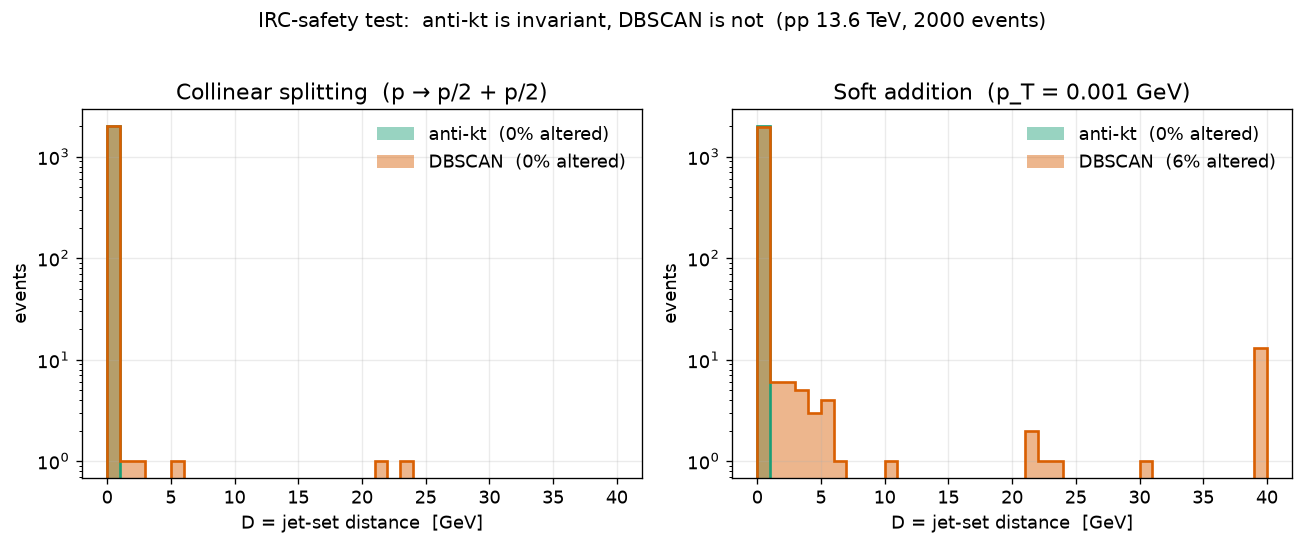
\includegraphics[width=\linewidth]{licao_irc_dbscan.png}
\caption{Jet-set distance $D$ [Eq.~\eqref{eq:D}] under a collinear splitting (left) and a
soft addition (right), for \antikt{} (green) and physical $(y,\phi)$ DBSCAN (orange), over
2000 events. \antikt{} is a delta function at $D=0$; DBSCAN develops a tail, most severely
in the infrared.}
\label{fig:dbscan}
\end{figure}

% ===========================================================================
\section{Restoring exact safety with energy weighting}
% ===========================================================================
The generalized-$\kt$ family underlying \antikt{} clusters particles by the inter-particle
and beam distances
\begin{equation}
d_{ij} = \min\!\big(p_{Ti}^{\,2p},\,p_{Tj}^{\,2p}\big)\,\frac{\Delta_{ij}^{2}}{R^{2}},
\qquad
d_{iB} = p_{Ti}^{\,2p},
\label{eq:genkt}
\end{equation}
repeatedly recombining the pair of smallest $d_{ij}$ (or calling $i$ a jet when $d_{iB}$ is
smallest), with $p=-1$ for \antikt{}, $p=0$ for Cambridge/Aachen~\cite{ca} and $p=+1$ for
the inclusive $\kt$ algorithm~\cite{kt}. Recombination uses the $E$-scheme, so a jet's
four-momentum and invariant mass are
\begin{equation}
p_J^{\mu} = \sum_{i\in J} p_i^{\mu},
\qquad
m_J^{2} = p_J^{\mu}p_{J\mu} = E_J^{2} - |\vec{p}_J|^{2}.
\label{eq:mass}
\end{equation}
The IRC safety of~\eqref{eq:genkt} is structural: a collinear pair has $\Delta_{ij}\to0$
and is recombined first, and a soft particle recombines with a nearby hard one before
influencing the hard jets.

\paragraph{Two networks.}
To ask whether a \emph{network} can be safe, we compare two permutation-invariant Deep-Sets
architectures~\cite{deepsets}, both of the generic form $\Obs = F\!\big(\sum_i\Phi(x_i)\big)$,
trained to regress the \antikt{} jet mass from the constituents expressed in coordinates
relative to the jet axis, $\hat y_i = y_i - y_J$, $\hat\phi_i = \phi_i - \phi_J$. The
\textbf{Energy Flow Network} (EFN)~\cite{efn} --- a nonlinear counterpart to the complete
linear basis of IRC-safe observables provided by energy flow polynomials~\cite{efp} ---
restricts the per-particle map $\Phi$ to
\emph{angular} information and weights it by the energy fraction:
\begin{equation}
\Obs_{\mathrm{EFN}} = F\!\left(\sum_{i} z_i\,\Phi(\hat y_i,\hat\phi_i)\right),
\qquad
z_i = \frac{p_{Ti}}{\sum_{j} p_{Tj}} .
\label{eq:efn}
\end{equation}
This form is IRC-safe by construction. Under the collinear splitting~\eqref{eq:coll} the
weight $z_i$ is shared between two identical angular arguments,
\begin{equation}
z_i\,\Phi(\hat y_i,\hat\phi_i)\;\longmapsto\;
z_i^{(1)}\Phi(\hat y_i,\hat\phi_i) + z_i^{(2)}\Phi(\hat y_i,\hat\phi_i)
= \big(z_i^{(1)}+z_i^{(2)}\big)\Phi(\hat y_i,\hat\phi_i)
= z_i\,\Phi(\hat y_i,\hat\phi_i),
\label{eq:efncoll}
\end{equation}
leaving the aggregate --- and hence $\Obs$ --- exactly invariant; and under the soft
emission~\eqref{eq:ir} the added term $z_{n+1}\Phi\to0$ as $z_{n+1}\propto\ptsoft\to0$,
recovering~\eqref{eq:scaling}.

As a deliberately unsafe control, the \textbf{Particle Flow Network} (PFN) lets $\Phi$ see
the energy fraction and aggregates with unit weight,
\begin{equation}
\Obs_{\mathrm{PFN}} = F\!\left(\sum_{i}\Phi(z_i,\hat y_i,\hat\phi_i)\right).
\label{eq:pfn}
\end{equation}
It violates both limits: a soft addition contributes a fixed
$\Phi(0,\hat y,\hat\phi)\neq0$ that does not vanish as $\ptsoft\to0$, and a collinear
splitting gives $\Phi(z^{(1)}\!,\cdot)+\Phi(z^{(2)}\!,\cdot)\neq\Phi(z,\cdot)$ because
$\Phi$ is nonlinear in $z$.

\subsection{Equal accuracy, unequal safety}\label{sec:equal}
Both networks share the same backbone (per-particle MLP $2/3\!\to\!128\!\to\!128\!\to\!128$,
latent dimension $128$, aggregation, and an MLP head), and are trained with
Adam for 80 epochs. On boosted jets they are statistically indistinguishable as mass
regressors (correlation $0.996$ vs $0.995$; Fig.~\ref{fig:efn}, Table~\ref{tab:efn}), yet
their behaviour under perturbation could not be more different (Table~\ref{tab:efn}). The
EFN is invariant to machine precision under collinear splitting in \emph{both} samples, and
its soft response is smaller than the PFN's by a factor of about $20$ on low-$\pt$ jets and
$\sim\!600$ on boosted jets. Crucially, the PFN's marginally better fit on the low-$\pt$
sample is obtained precisely by exploiting the IRC-unsafe information (soft counts,
collinear multiplicity) that its safe counterpart is forbidden to use.
The contrast is stable: over five random initializations (boosted sample) the EFN
correlation is $0.9959\pm0.0001$ and its soft response $0.010\pm0.000$~GeV, with the
collinear response identically zero in every run, whereas the PFN's soft response is not
only large but erratic, $9.1\pm2.1$~GeV (collinear $0.27\pm0.03$~GeV). The safe network is
reproducible in both accuracy and safety; the unsafe one is unstable in its very unsafety.

\begin{figure}[h]
\centering
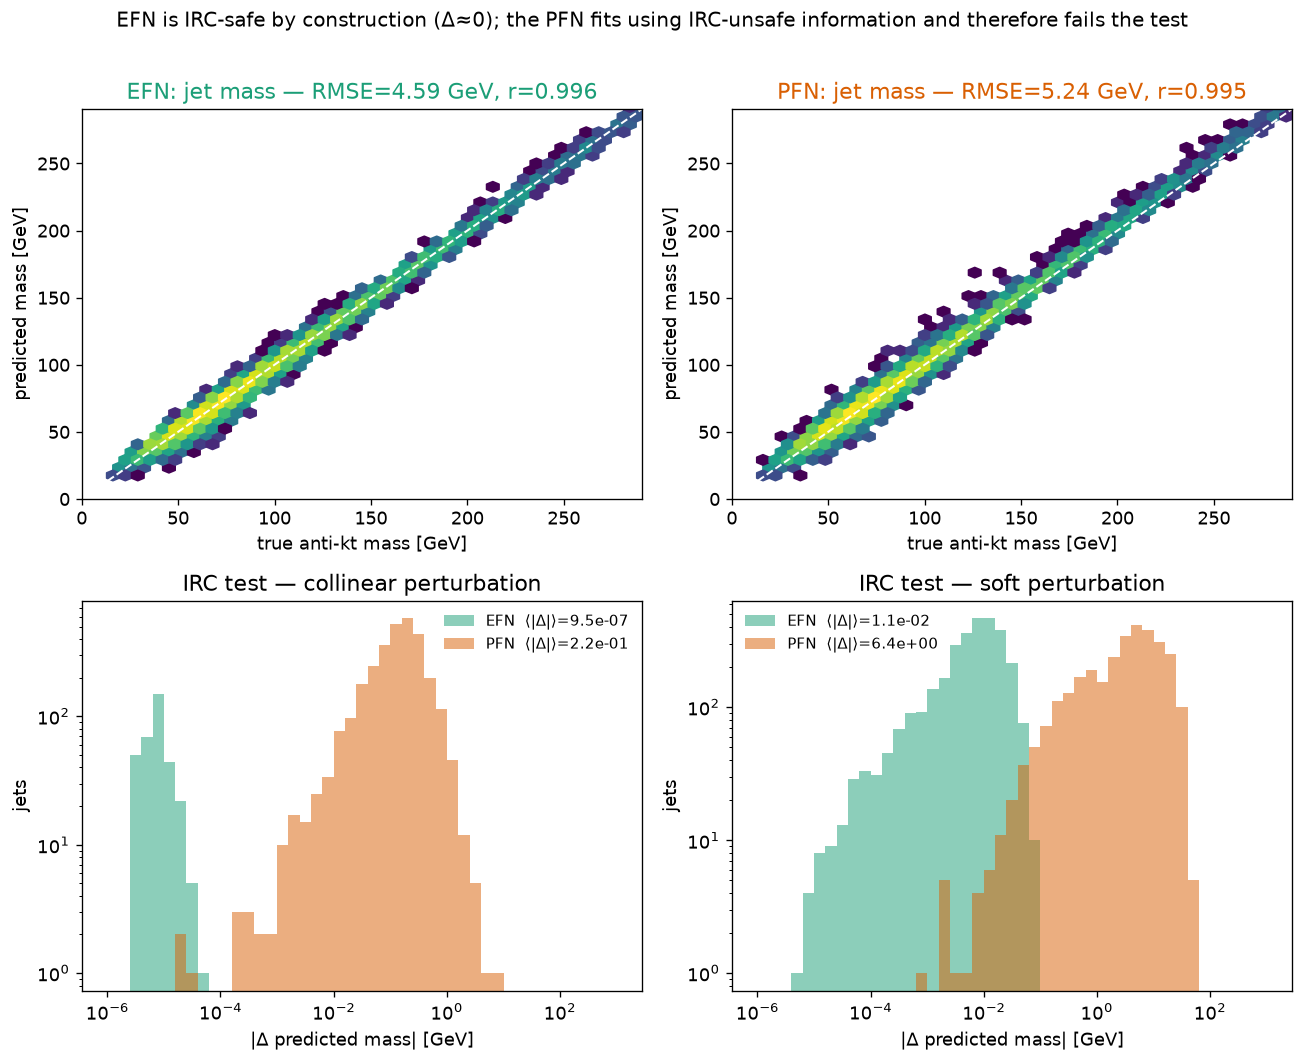
\includegraphics[width=\linewidth]{efn_resultados_boosted.png}
\caption{Boosted sample. Top: predicted vs.\ true \antikt{} jet mass for the EFN (left)
and PFN (right); both reach correlation $r\approx0.996$. Bottom: distribution of the induced
change $|\Delta m|$ under collinear (left) and soft (right) perturbations. The EFN piles up
at machine zero; the PFN spreads to several GeV.}
\label{fig:efn}
\end{figure}

\begin{table}[h]
\centering
\caption{Mass-regression accuracy and IRC response of the two networks. $|\Delta m|$ is the
mean induced mass change [GeV]; the collinear test uses $z=\tfrac12$, the soft test uses
$\ptsoft=10^{-3}$~GeV.}
\label{tab:efn}
\small
\begin{tabular}{lcccc}
\toprule
Model & corr & RMSE [GeV] & $|\Delta m|$ collinear & $|\Delta m|$ soft \\
\midrule
\multicolumn{5}{l}{\textit{Low-$\pt$ sample --- jet mass in GeV}}\\
EFN (\safe)   & 0.37 & 2.41 & \textbf{0.00000} & 0.133 \\
PFN (\unsafe) & 0.70 & 1.85 & 0.296            & 2.744 \\
\midrule
\multicolumn{5}{l}{\textit{Boosted sample --- jet mass in GeV}}\\
EFN (\safe)   & 0.996 & 4.59 & \textbf{0.00000} & 0.011 \\
PFN (\unsafe) & 0.995 & 5.25 & 0.225            & 6.429 \\
\bottomrule
\end{tabular}
\end{table}

\subsection{The scaling law is the proof}
A single perturbation size is suggestive; the limit is decisive. Figure~\ref{fig:scaling}
probes both limits over many decades. Under a soft emission (left) the EFN response falls as
a power law toward zero, reaching $1.4\times10^{-4}$~GeV at $\ptsoft=10^{-6}$~GeV, while the
PFN saturates at a plateau of $\approx2.6$~GeV that is independent of $\ptsoft$: the
contribution $\Phi(0,\cdot)$ of a zero-energy particle does not disappear. Under a collinear
splitting of opening angle $\theta$ (centre) the same pattern recurs --- the EFN vanishes as
a power law, falling faster than the linear reference (consistent with the leading
$\propto\theta^{2}$ behaviour expected when the two collinear daughters straddle the parent
symmetrically), whereas the PFN plateaus at $\approx0.29$~GeV. For an exactly collinear split
($\theta=0$, right) the EFN is invariant to machine precision ($\approx5\times10^{-8}$~GeV)
for every momentum fraction $z$; the PFN is not ($\approx0.3$~GeV). The vanishing of the EFN
response in \emph{both} limits is the operational content of
Eqs.~\eqref{eq:coll}--\eqref{eq:ir}; the PFN's two finite plateaus are the receipts of its
unsafety.

\begin{figure}[h]
\centering
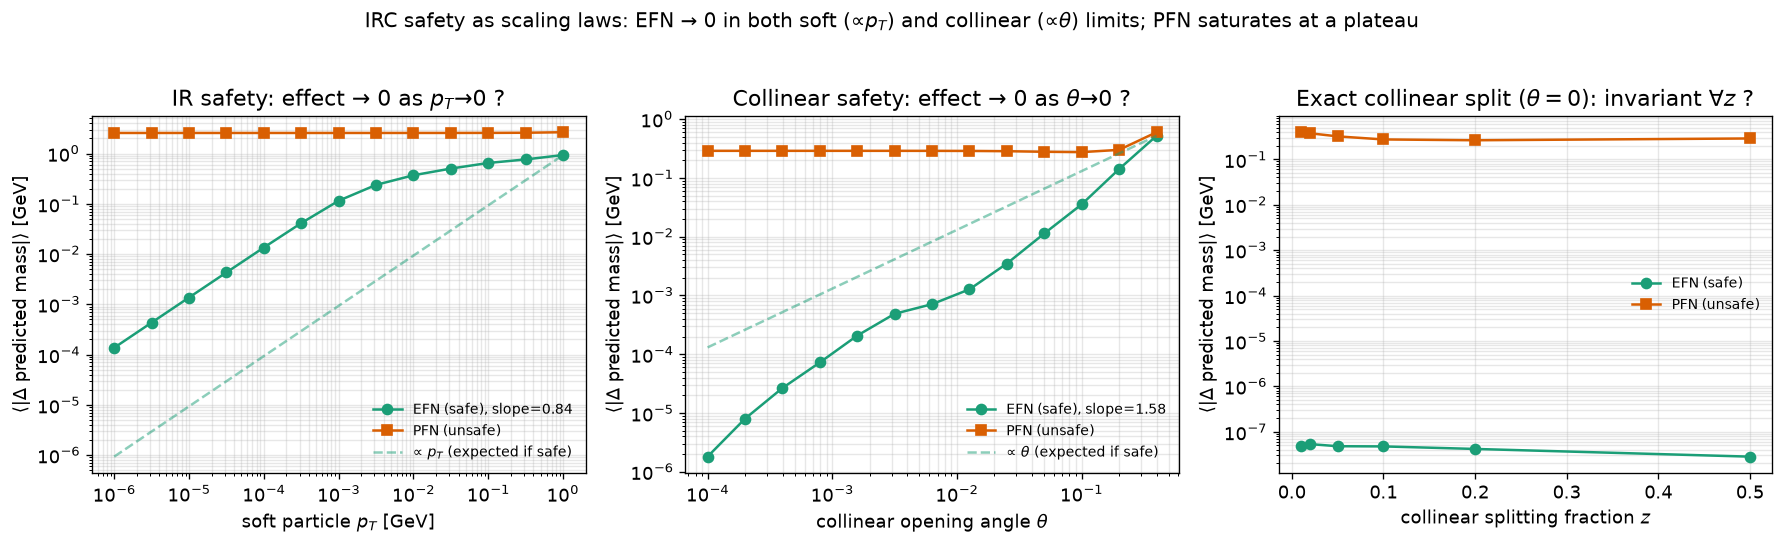
\includegraphics[width=\linewidth]{teste_irc_scaling.png}
\caption{IRC safety as scaling laws. Left: mean predicted-mass shift vs.\ the soft particle's
$\pt$ (log--log); the EFN vanishes as a power law, the PFN plateaus at $\approx2.6$~GeV.
Centre: shift vs.\ the collinear opening angle $\theta$; the EFN falls faster than the linear
reference toward zero, the PFN plateaus at $\approx0.29$~GeV. Right: shift vs.\ the
exactly-collinear momentum fraction $z$ ($\theta=0$); the EFN is flat at machine precision,
the PFN is not.}
\label{fig:scaling}
\end{figure}

% ===========================================================================
\section{A learned, provably safe jet algorithm}
% ===========================================================================
Sections~4--5 concern observables computed \emph{on} jets. We now make the clustering itself
learnable while keeping IRC safety exact, as a proof of concept within a low-dimensional but
provably safe family. Rather than a non-differentiable neural partition, we treat the
generalized-$\kt$ measure~\eqref{eq:genkt} as a two-parameter model --- energy exponent $p$
and radius $R$ --- and optimize it against a real physics objective on the boosted sample. Matching reconstructed jets to the outgoing hard partons (\textsc{Pythia}
status $\pm23$) within $\dR<0.35$, we define the energy response and its figure of merit
\begin{equation}
r = \frac{p_T^{\,\mathrm{jet}}}{p_T^{\,\mathrm{parton}}},
\qquad
b = \operatorname{median}(r) - 1,
\qquad
\sigma = \tfrac12\big(q_{84}-q_{16}\big),
\qquad
\mathcal{L}(p,R) = \sqrt{b^{2}+\sigma^{2}},
\label{eq:objective}
\end{equation}
where $b$ is the energy-scale bias, $\sigma$ the resolution (half the central $68\%$
interval of $r$), and $q_{\alpha}$ the $\alpha$-th percentile. The objective $\mathcal{L}$
has a genuine interior optimum: too small a radius misses final-state radiation ($b<0$),
too large a radius absorbs the underlying event ($b>0$). Every point of the scanned family
is a sequential-recombination algorithm and hence IRC-safe by construction --- the safety
is a hard constraint on the search space, not a term in the loss.

The optimum (Fig.~\ref{fig:phasea}, left) lands at $p^{\ast}=-1.0$, $R^{\ast}=1.0$: the
optimization \textbf{rediscovers the \antikt{} energy exponent} from scratch and prefers a
radius only slightly larger than the conventional $R=0.8$, improving the response RMS from
$\mathcal{L}=0.076$ to $0.073$. The exponent $p$ is weakly constrained by energy response
--- a quantitative statement of why \antikt's soft-resilient, rigid-cone behaviour is a
robust default. The IRC battery (Fig.~\ref{fig:phasea}, right; Table~\ref{tab:phasea})
confirms that the learned algorithm, together with the whole recombination family, has a
soft response of $\approx10^{-4}$~GeV --- consistent with floating-point noise --- while
DBSCAN sits nearly four orders of magnitude higher. Because the learned algorithm shares the
\antikt{} exponent at a larger radius, its jets fully contain the reference jets:
the constituent-$\pt$ overlap is $1.00$, and the mean jet mass rises from $88.9$ to
$117.1$~GeV as the wider jet captures more radiation.

\begin{figure}[h]
\centering
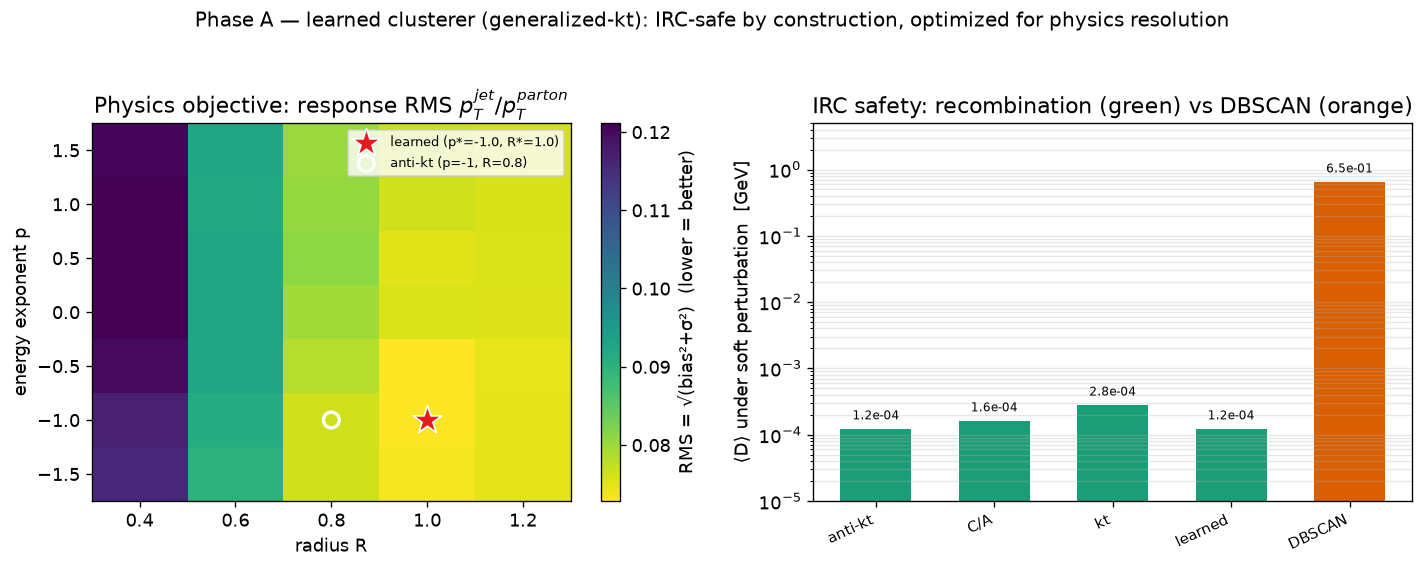
\includegraphics[width=\linewidth]{phase_a_genkt.png}
\caption{Left: the physics objective $\mathcal{L}(p,R)$ [Eq.~\eqref{eq:objective}] over the
generalized-$\kt$ family; the star marks the learned optimum
$(p^{\ast},R^{\ast})=(-1,1.0)$, the circle the \antikt{} reference. Right: mean
soft-perturbation distance $\langle D\rangle$ per algorithm (log scale); all
sequential-recombination algorithms (green) are safe, DBSCAN (orange) is not.}
\label{fig:phasea}
\end{figure}

\begin{table}[h]
\centering
\caption{Learned generalized-$\kt$ vs.\ the \antikt{} $R=0.8$ reference on boosted jets.
The learned jets fully contain the \antikt{} jets (constituent-$\pt$ overlap $=1.00$),
being the same exponent at a larger radius.}
\label{tab:phasea}
\small
\begin{tabular}{lcccccc}
\toprule
Algorithm & RMS resp.\ $\mathcal{L}$ & bias $b$ & $\sigma$ & jets/event &
mean mass [GeV] & $\langle D\rangle$ soft [GeV] \\
\midrule
\antikt{} \, ($p=-1,\,R=0.8$)   & 0.076 & $0.000$  & 0.076 & 2.18 & 88.9  & 0.0001 \\
learned \, ($p^\ast=-1,\,R^\ast=1.0$) & \textbf{0.073} & $+0.010$ & \textbf{0.072} & 2.16 & 117.1 & 0.0001 \\
DBSCAN \, ($\varepsilon=0.8$)   & ---   & ---      & ---   & ---  & ---   & 0.6453 \\
\bottomrule
\end{tabular}
\end{table}

% ===========================================================================
\section{Discussion}
% ===========================================================================
The three studies form a single argument. DBSCAN shows that adopting a generic clustering
method imports its symmetries --- and density has the wrong ones. The EFN--PFN pair isolates
the mechanism: two networks of equal expressive power and near-identical accuracy diverge
completely in safety, decided entirely by whether energy enters as a linear weight
[Eq.~\eqref{eq:efn}, safe] or as a feature summed with unit weight [Eq.~\eqref{eq:pfn},
unsafe]. The scaling law~\eqref{eq:scaling} elevates this from ``small vs.\ large'' to the
exact limit that defines the property. Finally, the learned algorithm shows the constructive
route: parametrize \emph{within} a provably safe family and let optimization choose --- here
recovering \antikt's exponent and quantifying the mild preference for a larger radius once
the underlying event is present.

Limitations are worth stating plainly. The learnable clustering explores a two-parameter
family, not an arbitrary neural partition; extending learnable safe clustering to a richer,
still-safe hypothesis class --- for instance an energy-weighted, permutation-equivariant
metric inside the recombination loop --- is the natural next step. The jet-mass regression
targets a single observable; the EFN's low correlation on low-$\pt$ jets is itself physical
--- at that scale the IRC-safe information content of the mass is genuinely small --- and it
rises to $0.996$ once the mass becomes a real scale. All results are at particle level
without detector effects or pileup, whose interaction with IRC safety is an important
separate axis. Finally, all quoted numbers derive from the finite samples of
Table~\ref{tab:samples}; the sensitivity of the network results to initialization is
quantified in Sec.~\ref{sec:equal}, and the central claim of the scaling laws --- exact
vanishing versus a finite plateau --- does not depend on sample size.

\paragraph{Takeaway.}
IRC safety is an exact symmetry of the physics, not a statistic. A model is safe only if its
\emph{architecture} makes it so --- energy weighting for observables, sequential
recombination for clustering. Imposed as a constraint it costs essentially nothing; chased
as a training target it is never actually reached, and the plateau in Fig.~\ref{fig:scaling}
is the receipt.

% ===========================================================================
\section{Conclusions}
% ===========================================================================
We provided a quantitative, reusable battery for testing infrared and collinear safety of
jet algorithms and machine-learning models, and used it to (i) diagnose density-based
clustering as IRC-unsafe, (ii) demonstrate that energy-weighted Deep-Sets restore exact
safety at no cost in accuracy, with the soft-momentum scaling law~\eqref{eq:scaling} as
rigorous proof, and (iii) construct a learnable jet algorithm that is IRC-safe by
construction and rediscovers the \antikt{} exponent when optimized against jet--parton
energy response. The through-line for physics-oriented machine learning is that exact
symmetries belong in the function class, not in the loss.

\paragraph{Reproducibility.}
All results were produced on a single CPU (Intel i5-13450HX) with \textsc{Pythia}~8.317,
\textsc{FastJet}~3.5.1, PyTorch~2.12.1 (CPU)~\cite{pytorch}, scikit-learn~1.9.0~\cite{sklearn},
NumPy~2.2.4 and Python~3.13. The pipeline is fully scripted and seeded:
\texttt{gerar\_dados.py} (generation and \antikt{} reference), \texttt{licao\_irc\_dbscan.py}
(Fig.~\ref{fig:dbscan}), \texttt{efn.py} (EFN/PFN training, Fig.~\ref{fig:efn},
Table~\ref{tab:efn}), \texttt{teste\_irc\_scaling.py} (Fig.~\ref{fig:scaling}), and
\texttt{phase\_a\_genkt.py} (Fig.~\ref{fig:phasea}, Table~\ref{tab:phasea}). The EFN predicts
the dimensionless ratio $m/\pt$ on boosted jets and is rescaled by the (IRC-safe) jet $\pt$.

% ===========================================================================
\begin{thebibliography}{99}
\bibitem{antikt} M.~Cacciari, G.~P.~Salam, G.~Soyez,
  \emph{The anti-$k_t$ jet clustering algorithm}, JHEP \textbf{04} (2008) 063,
  arXiv:0802.1189.
\bibitem{fastjet} M.~Cacciari, G.~P.~Salam, G.~Soyez,
  \emph{FastJet user manual}, Eur.\ Phys.\ J.\ C \textbf{72} (2012) 1896, arXiv:1111.6097.
\bibitem{kt} S.~D.~Ellis, D.~E.~Soper,
  \emph{Successive combination jet algorithm for hadron collisions},
  Phys.\ Rev.\ D \textbf{48} (1993) 3160, arXiv:hep-ph/9305266.
\bibitem{ca} Y.~L.~Dokshitzer, G.~D.~Leder, S.~Moretti, B.~R.~Webber,
  \emph{Better jet clustering algorithms}, JHEP \textbf{08} (1997) 001, arXiv:hep-ph/9707323.
\bibitem{efn} P.~T.~Komiske, E.~M.~Metodiev, J.~Thaler,
  \emph{Energy Flow Networks: Deep Sets for particle jets}, JHEP \textbf{01} (2019) 121,
  arXiv:1810.05165.
\bibitem{deepsets} M.~Zaheer, S.~Kottur, S.~Ravanbakhsh, B.~P\'oczos, R.~Salakhutdinov,
  A.~Smola, \emph{Deep Sets}, NeurIPS \textbf{30} (2017), arXiv:1703.06114.
\bibitem{pythia} C.~Bierlich et al.,
  \emph{A comprehensive guide to the physics and usage of PYTHIA 8.3},
  SciPost Phys.\ Codebases \textbf{8} (2022), arXiv:2203.11601.
\bibitem{salam} G.~P.~Salam, \emph{Towards jetography},
  Eur.\ Phys.\ J.\ C \textbf{67} (2010) 637, arXiv:0906.1833.
\bibitem{dbscan} M.~Ester, H.-P.~Kriegel, J.~Sander, X.~Xu,
  \emph{A density-based algorithm for discovering clusters in large spatial databases with
  noise}, Proc.\ KDD-96 (1996) 226.
\bibitem{efp} P.~T.~Komiske, E.~M.~Metodiev, J.~Thaler,
  \emph{Energy flow polynomials: a complete linear basis for jet substructure},
  JHEP \textbf{04} (2018) 013, arXiv:1712.07124.
\bibitem{sterman} G.~Sterman, S.~Weinberg, \emph{Jets from quantum chromodynamics},
  Phys.\ Rev.\ Lett.\ \textbf{39} (1977) 1436.
\bibitem{pytorch} A.~Paszke et al.,
  \emph{PyTorch: an imperative style, high-performance deep learning library},
  NeurIPS \textbf{32} (2019), arXiv:1912.01703.
\bibitem{sklearn} F.~Pedregosa et al.,
  \emph{Scikit-learn: machine learning in Python}, JMLR \textbf{12} (2011) 2825.
\end{thebibliography}

\end{document}
